\chapter{Biofilter modeling}\label{ch03_bio}

The nuclear pore complex (NPC) is a biofilter that blocks certain macromolecules
while allowing the passage of others. Binding is crucial: transport factors (TF)
that can bind to disordered proteins (FG nucleoporins or FG nups) in the NPC
move through rapidly~\cite{strambio-de-castillia_nuclear_10}.  Other examples of
biofilters that facilitate transport of nanoparticles, like proteins and
viruses, are the pericellular matrix in cells, the extracellular matrix in
tissues, mucus in cells, and synthetic hydrogels~\cite{witten_particle_17}.  In
certain cases, binding can reduce the transport of macromolecules across the
filter, which has negative implications for drug delivery, \textit{e.g.}, cancer
treatments can bind to mucosal layers~\cite{witten_particle_17}. In other
circumstances, the role of binding is protective, \textit{e.g.}, mucus trapping
viruses and other nanoparticles~\cite{schneider_fluorescent_17,
  huang_protein_17, mastorakos_highly_15}. Binding and bound mobility play a
role in selectivity in all these biofilters.

Laura Maguire, Meredith Betterton, Loren Hough, and I developed a general
framework to study transport across the NPC, and the model can be applied to
other biofilters.  The collaboration originally formed to model experimental
density profiles of a hydrogel NPC mimic created in the Hough lab. Focus shifted
to a theory paper summarized in \cref{maguire_design_18}.  My role was mainly
focused on numerically evaluating the model's continuum equations while Laura
Maguire worked on different bound motion mechanisms.

The work in the previous chapter stressed the importance of inhomogeneities that
cause anomalous diffusion.  In this chapter, we study transport across
biofilters by analyzing the bulk-continuum behavior of particle concentration.
We assume that obstacles form a homogeneous continuum in which tracers can bind
at any given location.  Once bound, a tracer may also exhibit bound motion. 

% figure01 %
\begin{figure}[!t]
  \begin{center}
    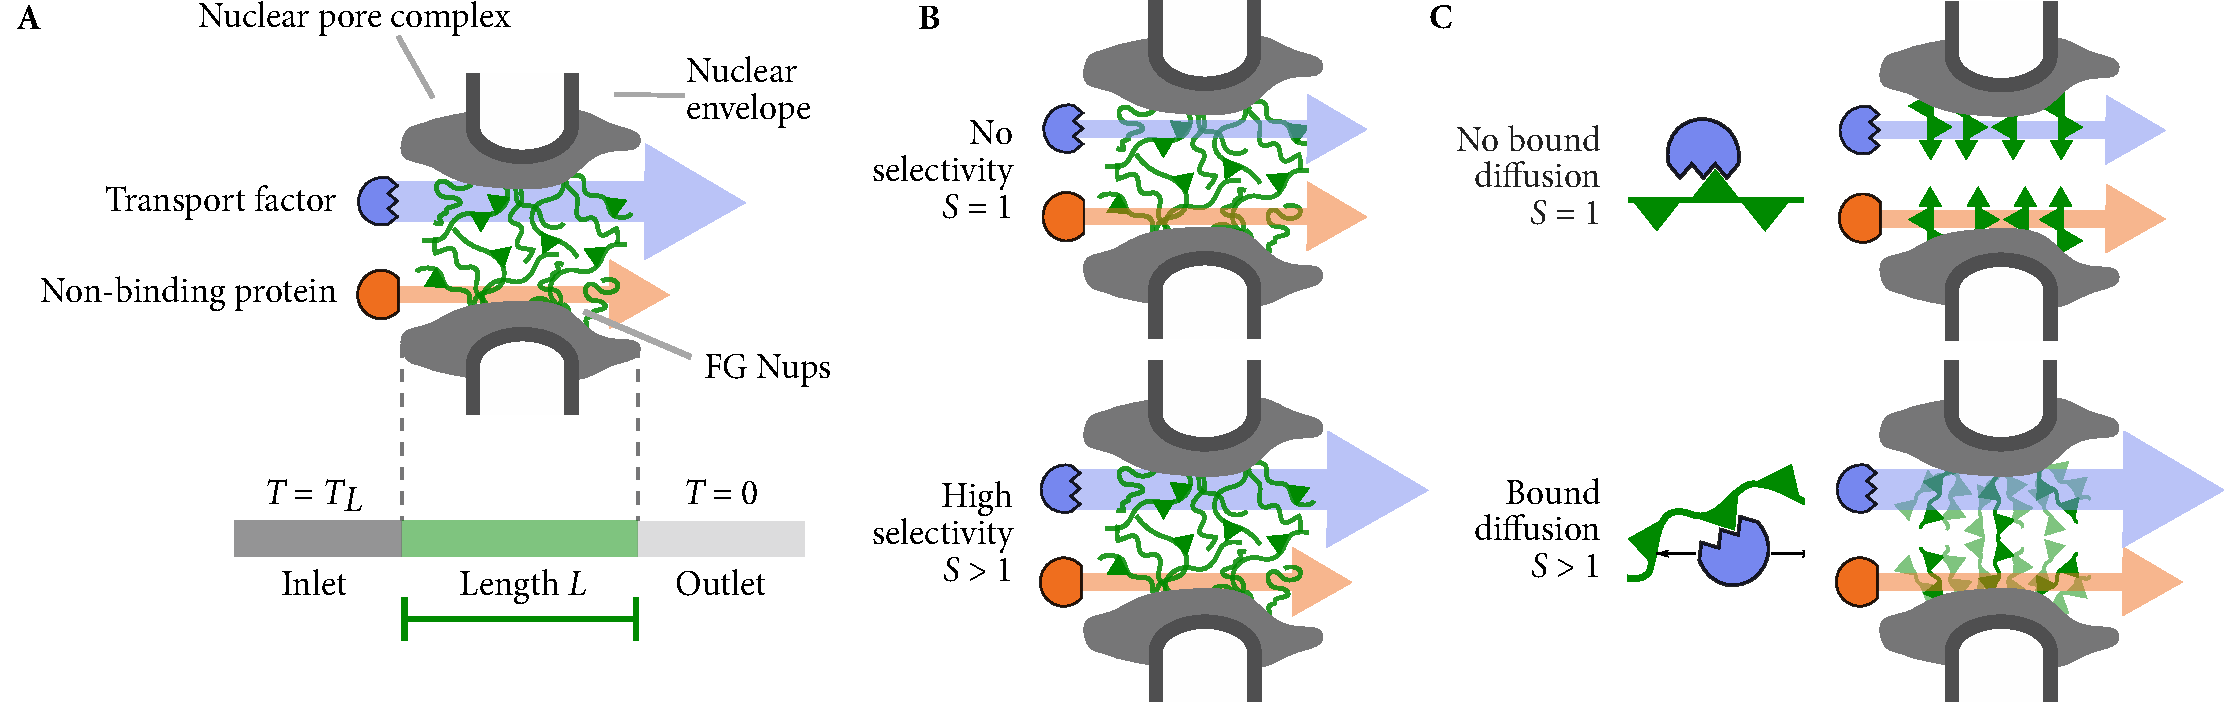
\includegraphics[width=150mm]{figs/ch03_bio/bio_cartoon.pdf}
  \end{center}
	\caption[NPC model schematic]
  {Schematics of the nuclear-pore complex and model. (A) The
  nuclear pore complex (gray) is filled with FG Nups (green polymers)
  that selectively passage transport factors that bind to FG Nups
  (blue) while blocking non-binding proteins (red). The central
  channel of the pore has length $L$. Protein concentration is high on
  the left (inlet) and low on the right (outlet).  (B) Selectivity
  quantifies the degree of selective transport through the pore. A
  non-selective pore with $S=1$ has the same flux for a transport
  factor as for a non-binding protein (top). A selective pore with
  $S>1$ has a larger flux for a transport factor than a non-binding
  protein (lower). (C) The bound diffusion coefficient quantifies the
  mobility of a bound transport factor.  A transport factor may be
  immobile (top) or mobile (lower) when bound. Figure created by Laura Maguire
  and used with permission.}\label{fig:bio_cartoon}
\end{figure}
% figure01 %

\section{Reaction-diffusion model of selectivity in biofilters}

In this section, we present a minimal model that can be used to characterize
transport across biofilters and apply this tool to study selectivity in the NPC
\figrefp{fig:bio_cartoon}.  Particles diffuse with coefficient $D_F$ in a
one-dimensional gel of length $L$.  The gel is filled with binding sites at
concentration $N_T$ with a binding on-rate constant $\kon$, off-rate $\koff$,
and dissociation constant $K_D = \frac{\koff}{\kon}$.  In the NPC, these binding
sites correspond to polymers  that some proteins (TF) bind to while others
cannot.  The free species has concentration $T$ while the bound species has
concentration $C$.  The concentration of the inlet and outlet for the free
species are fixed to $T_L$ and $0$, respectively.  Once bound, the  complex can
diffuse ($D_B$).  Since the binding sites are immobile, the bound species has
no-flux boundary conditions.  The number of free binding sites is $N(x) = N_T -
C(x)$. We assume that particles do not interact with each other.  This system is
described by the reaction diffusion equations
%
\begin{eqnarray}
\label{eqn:continuum_main} 
  \frac{\partial T}{\partial t} &=& 
  -\kon T N+\koff C +D_F
       \frac{\partial^2 T}{\partial x^2},
   \\ 
\label{eqn:continuum_main_2} 
  \frac{\partial C}{\partial t} &=& \kon T N -\koff C + 
        D_B \frac{\partial^2 C}{\partial x^2}.
\end{eqnarray}
%
The second two terms in \eqn~\ref{eqn:continuum_main}
and~\ref{eqn:continuum_main_2} correspond to reaction kinetics while the last
term describes diffusion.  The bound complex (a particle bound to a site)
diffuses, meaning, a bound particle can move across binding sites without
unbinding.  We chose a parameter set that described the NPC
\tablerefp{table:parameters}. 

% table01 %
\begin{table}[!b]
  \begin{center}
    %\begin{tabular}{p{1.7cm}p{0.75cm}p{1.1cm}p{0.7cm}p{0.8cm}p{0.8cm}}
    \begin{tabular}{p{3.00cm}p{2.0cm}p{3.0cm}p{3.0cm}}
      Parameter & Symbol & Value & Notes\\
      \toprule
      Box length & $L$ & $100 \, \nm $ 
      &~\cite{frenkiel-krispin_structural_10, maimon_human_12}\\
      Free diffusion  & $D_F$ & $0.012 \,\mu \tx{m}^2 $/s
      &Calculated from flux~\cite{ribbeck_kinetic_01}\\
      Bound diffusion  & $D_B/D_F$ &  $0$--$1$
      &Our model~\cite{maguire_design_18}\\
      Binding on-rate  & $k_{\tx{on}}$  &  $10^{-9} \, \tx{Ms}^{-1}$
      &Diffusion-limited~\cite{milles_plasticity_15, hough_molecular_15}\\
      Inlet concentration  & $T_L$& $ 1 \, \mu$M
      &Calculated bulk concentration of $5 \, \mu$M an 
      estimated barrier height of
      1.5 $k_B T$~\cite{timney_simple_16}  \\
      Dissociation constant  & $K_D$& $ 10^{-2}$--$10^{3}\,\mu$M
      &~\cite{pyhtila_gradient_03, gilchrist_accelerating_02, tetenbaum-novatt_nucleocytoplasmic_12, milles_plasticity_15, timney_simple_16, vovk_simple_16} \\
      Binding site concentration  & $N_T$ & $4700 \,\mu$M
      &Estimate of $800$ binding sites with $60 \, \nm$ pore diameter 
      \\
    \end{tabular}
  \end{center}
  \caption[NPC parameters]
  {The parameters we used to model the NPC\@.}\label{table:parameters}
\end{table}
%
The particle flow into the outlet is given by the flux, $J = -D_F
\diff{T}{x}|_{x=L}$.  As particles diffuse across the gel, the flux reaches
steady state.  We define the selectivity as 
%
\begin{equation}
  \label{eqn:selectivity}
  S =  \frac{J_{\rm binding}(t \to \infty)}{J_{\rm non-binding}(t \to \infty)}.
\end{equation}
%
The selectivity is the flux into the outlet at steady state relative to the flux
of a non-binding particle.  A filter is selective if it has the ability to let
certain particles through while blocking others. 

\subsection{Linear solution and numerics}\label{sec:numerics_and_properties}

The steady state solution in the absence of binding is
%
\begin{equation}
\label{eqn:linear_steady}
  T(x) = \frac{T_L (L-x)}{L}; \qquad J = \frac{D_F T_L}{L}.
\end{equation}
%
When $D_B=0$, the unbound species steady state concentration is linear
\eqnrefp{eqn:linear_steady}.  When bound motion does not occur, the reaction
kinetics do not play a role in selectivity.  While kinetics cannot alter the
steady state density profile, it can influence dynamics.

When $C(x)/N_T$ is small compared to one, the model is approximately linear.
Physically, this corresponds to binding site saturation.  A linear model assumes
that binding sites can always accept another binding complex.  This can lead to
unphysical results if the concentration of the bound complex exceeds the
concentration of binding sites.  At chemical equilibrium,
%
\begin{equation}
  C \koff  =  \kon A (N_T - C ).
\end{equation}
%
The linearity condition is then
%
\begin{equation}
  \frac{C(x)}{N_T} = \frac{1}{K_D / T(x) + 1} \ll 1.
\end{equation}
% 
The maximum concentration of the free species occurs at the boundary where
$T=T_L$.  Therefore, our system is linear when
%
\begin{equation}
  \label{eqn:rd_linear_cond}
  \frac{T_L}{K_D} \ll 1.
\end{equation}
%
When this condition is met, we can drop the non-linear term in the coupled
reaction-diffusion equations. We can solve for the linear solution of the free
species
%
\begin{equation}
  \label{eqn:rd_linear_sol}
  T(x) = b + m x + f e^{\lambda x} + g e^{-\lambda x},
\end{equation}
%
where $\lambda^2 = \koff(D_F+ N_t K_A D_B)/(D_F D_B)$ and $b, m, f, g$ are
coefficients fixed from boundary conditions~\cite{maguire_design_18}.

The coupled reaction-diffusion equations can be written
%
\begin{equation}
\frac{\partial \bm{a}}{\partial t} = L_{\text{op}} \bm{a} 
+ W_{\text{op}}(\bm{a}),
\end{equation}
%
where $\bm{a} = [T(x), \, C(x)]'$, $W_{\text{op}}(\bm{a}) = [\kon T(x) C(x), \,
-\kon T(x) C(x)]'$ a non-linear function of $\bm{a}$, and the linear operator
is
% 
\begin{equation}
L_{\text{op}} = 
  \begin{bmatrix}
    D_F\secdiff{}{x}-\kon N_T & \koff \\
    \kon N_T & D_B\secdiff{}{x}-\koff \\
  \end{bmatrix}.
\end{equation}
%
We used finite differences to approximate the second derivative
%
\begin{equation}
  \left. \secdiff{f}{x}\right|_{x_i} = \frac{f_{i+1} - 2f_{i} + f_{i-1}}{\delta x^2},
\end{equation}
%
where $f_i=f(x_i)$ is the function evaluated at the $i^{\tx{th}}$ grid point and
$\delta x$ the grid spacing.  We can break up the operators into block
matrices that act on $T$, $C$, and coupling terms as
%
\begin{equation}
L_{\tx{op}} =
\left[
\begin{array}{c c c}
  L^{T}_{\tx{op}}  & \rvline &  L^{C\rightarrow T}_{\tx{op}}\\
\midrule
L^{T\rightarrow C}_{\tx{op}}  & \rvline & L^{C}_{\tx{op}}
\end{array}
\right].
\end{equation}
%
The linear operator that acts on $T$ is
%
\begin{equation}
L^{T}_{\tx{op}} =
\begin{bmatrix}
  0 & 0 & 0 & \cdots & 0 & 0 \\
  \frac{D_F}{\delta x^2} & -\kon N_T -\frac{2 D_F}{\delta x^2} &
  \frac{D_F}{\delta x^2} & \cdots & 0 & 0\\
  0 & \frac{D_F}{\delta x^2} & -\kon N_T -\frac{2 D_F}{\delta x^2} &  \cdots & 0 & 0\\
  \vdots & & &\ddots \\
  0 & \cdots & 0 &\frac{D_F}{\delta x^2} & -\kon N_T -\frac{2 D_F}{\delta x^2}  & \frac{D_F}{\delta x^2}\\
  0 & 0 & 0 & \cdots & 0 & 0 \\
\end{bmatrix}.
\end{equation}
%
Note, the first and last row are zero because of Dirichlet boundary conditions.
The operator that acts on $C$ is
%
\begin{equation}
L^{C}_{\tx{op}} =
\begin{bmatrix}
  -\koff -\frac{2 D_B}{\delta x^2} &
  \frac{2D_B}{\delta x^2} & 0 &\cdots & 0 & 0\\
  \frac{D_B}{\delta x^2} &-\koff -\frac{2 D_B}{\delta x^2} &
  \frac{D_B}{\delta x^2} & \cdots & 0 & 0\\
  0 & \frac{D_B}{\delta x^2} & -\koff -\frac{2 D_B}{\delta x^2} &  \cdots & 0 & 0\\
  \vdots & & &\ddots & \\
  0 & \cdots & 0 & \frac{D_B}{\delta x^2} & -\koff -\frac{2 D_B}{\delta x^2}  & \frac{D_B}{\delta x^2}\\
  0 & 0 & 0 & \cdots & \frac{2 D_B}{\delta x^2} & -\koff -\frac{2 D_B}{\delta x^2} \\
\end{bmatrix},
\end{equation}
where now Neumann boundary conditions are enforced. The coupling matrices are
given by
% Noise
\begin{gather}
  L^{C\rightarrow T}_{\tx{op}} = \koff \mathbb{I}, \\
  L^{T\rightarrow C}_{\tx{op}} = \kon N_T \mathbb{I},
\end{gather}
%
where $\mathbb{I}$ is the identity operator.  Our numeric scheme evolves the
linear term with a Crank-Nicolson step and the nonlinear term with an Euler
step,
%
\begin{equation}
  \bm{a}_{n+1} = \bm{a}_n + \delta t L_{op} (\bm{a}_n + \bm{a}_{n+1})/2 
  + W_{op}(\bm{a}_n) \delta t,
\end{equation}
%
where $n$ refers to the $n^{\tx{th}}$ time step.  This can be rearranged to give
%
\begin{equation}
  \bm{a}_{n+1} = {\left(\mathbb{I} - \frac{\delta t}{2} L_{op}\right)}^{-1}
  \left( \left[\mathbb{I} + \frac{\delta t}{2} L_{op}\right] \bm{a}_n 
  + W_{op}(\bm{a}_n) \delta t \right).
\end{equation}
%
The numerical integration was implemented in \textsc{matlab}. For a computation
speed-up, the \textsc{matlab} function \textit{mldivide} was used instead of
inverting any matrices.  We also numerically found steady state solutions of the
equation
%
\begin{equation}
  \label{eqn:ode}
  \diff{}{x}
  \begin{bmatrix}
    T \\
    C \\
    T_x \\
    C_x 
  \end{bmatrix}
  =
  \begin{bmatrix}
    T_x  \\
    C_x \\
    \frac{1}{D_F} \left[ \kon T ( N_T - C ) - \koff C  \right] \\
    -\frac{1}{D_B} \left[ \kon T ( N_T - C ) - \koff C  \right] \\
  \end{bmatrix},
\end{equation}
%
where the $x$ subscript refers to partial differentiation with respect to $x$,
using the differential equation solver bvp5c in \textsc{matlab}.  Whenever we
were interested in the dynamics, we solved the full PDE\@; all of the
selectivity measurements were found by numerically integrating the ODE
\eqnrefp{eqn:ode}.


\section{Selectivity in the nuclear pore}

% figure02 %
\begin{figure}[!t]
  \begin{center}
    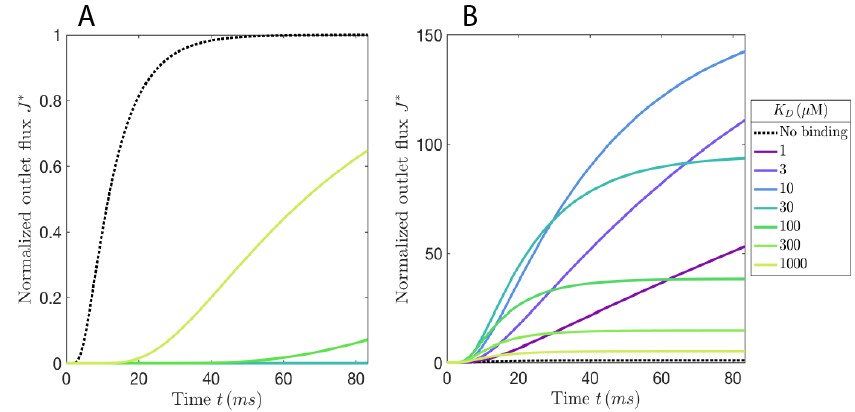
\includegraphics[width=150mm]{figs/ch03_bio/biofilter_jvst.png}
  \end{center}
	\caption[Transient flux]
  {Transient flux with (A) no bound motion ($D_B = 0$) and (B) bound motion 
    ($D_B=1$).}\label{fig:bio_jvst}
\end{figure}
% figure02 %

The transient behavior was found for no bound mobility \figrefp[A]{fig:bio_jvst}
and bound mobility \figrefp[B]{fig:bio_jvst}. Note the different axis limits.
Without bound mobility, binding slowed transport, and there was no selectivity.
For $D_B > 0$, there was a large increase in particle flux, and particles moved
more quickly through the gel. 

% figure %
\begin{figure}[!b]
  \begin{center}
    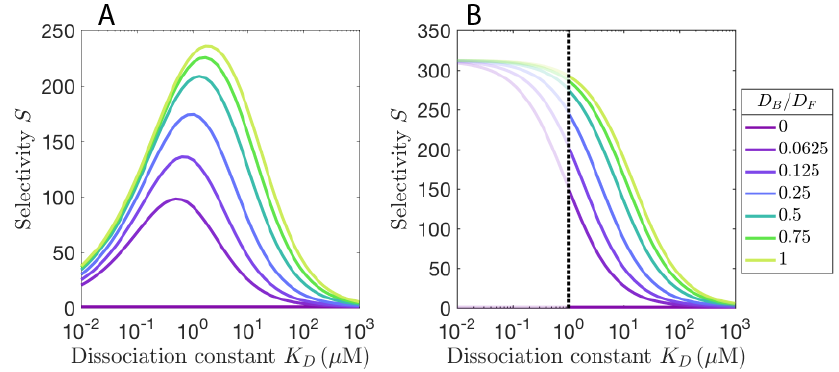
\includegraphics[width=150mm]{figs/ch03_bio/biofilter_sel.png}
  \end{center}
	\caption[Selectivity versus dissociation constant]
  {Selectivity as a function of diffusion coefficient
  ratio, with varying dissociation constant using the (A)
  full model and (B) linear approximation.}\label{fig:bio_sel}
\end{figure}
% figure %

In the model, increasing the bound diffusion coefficient always increases
selectivity \figrefp{fig:bio_sel}.  Varying binding leads to a non-monotonic
change of selectivity in the full model \figrefp[A]{fig:bio_sel}.  In the weak
binding limit $K_D \sim 10^3 \, \mu$M, decreasing $K_D$ increases selectivity.
As more particles bind, larger gradients in $T(x)$ form, and selectivity
increases.  As binding increases further $K_D < 1 \, \mu$M, the binding sites
saturate $N(x) \sim N_T$.  Saturation mitigates the inhomogeneity, and
therefore, lowers selectivity.

We investigated the non-linear coupling term $T(x)C(x)$
(\eqn~\ref{eqn:continuum_main},~\ref{eqn:continuum_main_2}) by comparing the
full \figrefp[A]{fig:bio_sel} and linear solutions \figrefp[B]{fig:bio_sel}.
The peak in selectivity in the full model occurs near the linear threshold $K_D
\sim 1\mu$M. Finally, we found that our model corresponds to experimental
selectivity measurements \tablerefp{table:NTF2-flux}. The results are for two
similarly size proteins: NTF2 (can bind) GFP (cannot bind). Our model captures
the range of selectivity values for the NPC\@.
% table01 %
\begin{table}[!b]
  \begin{center}
    \begin{tabular}{p{2.7cm}p{1.75cm}p{2.75cm}p{1.75cm}p{1.75cm}p{1.75cm}}
      Method & Cell type & Species & Flux & Selectivity & Notes\\
      \toprule
      OSTR & \textit{Xenopus} & \makecell[cl]{NTF2\\GFP} & 
      \makecell[cl]{91--123\\3.3--3.8} & 24--37 &\cite{siebrasse_rapid_02} \\
      OSTR & \textit{Xenopus} & \makecell[cl]{NTF2\\GFP} &
      \makecell[cl]{47.3\\1.1} & 43 &~\cite{kiskin_optical_03}\\
      \makecell[cl]{Permeabilized \\ cells}  & HeLa &
      \makecell[cl]{NTF2\\GFP} &
      \makecell[cl]{250\\2} & 125 &~\cite{ribbeck_kinetic_01}\\
      Model & --- & \makecell[cl]{Binding\\Non-binding} & 
      \makecell[cl]{2--480\\2} & 1--240 & \makecell[cl]{This\\work}\\
    \end{tabular}
  \end{center}
  \caption[Selectivity comparison between experiment and model]
  {Comparison between experimental results for NTF2 and GFP
    (a similarly-sized non-binding protein) and model
    predictions. Flux measured in units of molecules per pore per
    second. Table made by Laura Maguire and 
    used with permission}\label{table:NTF2-flux}
\end{table}

\subsection{Comparison to lattice model}

How does this system correspond to the previous lattice model
(Chapter~\ref{ch02_soft})?  In that model, inhomogeneities introduced memory
effects that caused anomalous diffusion, and obstacles excluded volume at
specific locations. Here, particles can bind anywhere, and obstacles cannot
block a specific step.  Rather, there is a chance that a tracer will bind at a
given time step without changing its position.  We can image this as a
dual-lattice system: one lattice corresponds to a free state and another
corresponds to a bound state.  When free, a particle undergoes a random walk on
the free-state lattice.  There is a probability to bind to the other lattice.
When it does, it stays at the same position but moves onto the bound-state
lattice.  Similarly, it can hop back to the free-state from the bound-state
lattice.  These binding probabilities correspond to $\kon$ and $\koff$, and
differing step rates on the lattices are related to the diffusion coefficients.
